\section{Reinforcement Learning for Reasoning Skill Refinement}
\begin{frame}[allowframebreaks]{}
    \LARGE Reinforcement Learning for Reasoning Skill Refinement
\framebreak
    \begin{figure}[h]
        \centering
        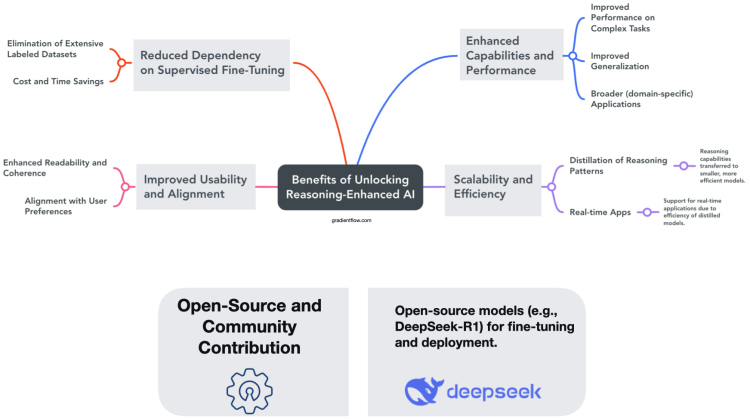
\includegraphics[width=\textwidth,height=0.9\textheight,keepaspectratio]{images/lrm+moe/rl-rsr.png}
    \end{figure}
\end{frame}

\begin{frame}[allowframebreaks]{Reinforcement Learning for Reasoning Skill Refinement}
    \begin{figure}[h]
        \centering
        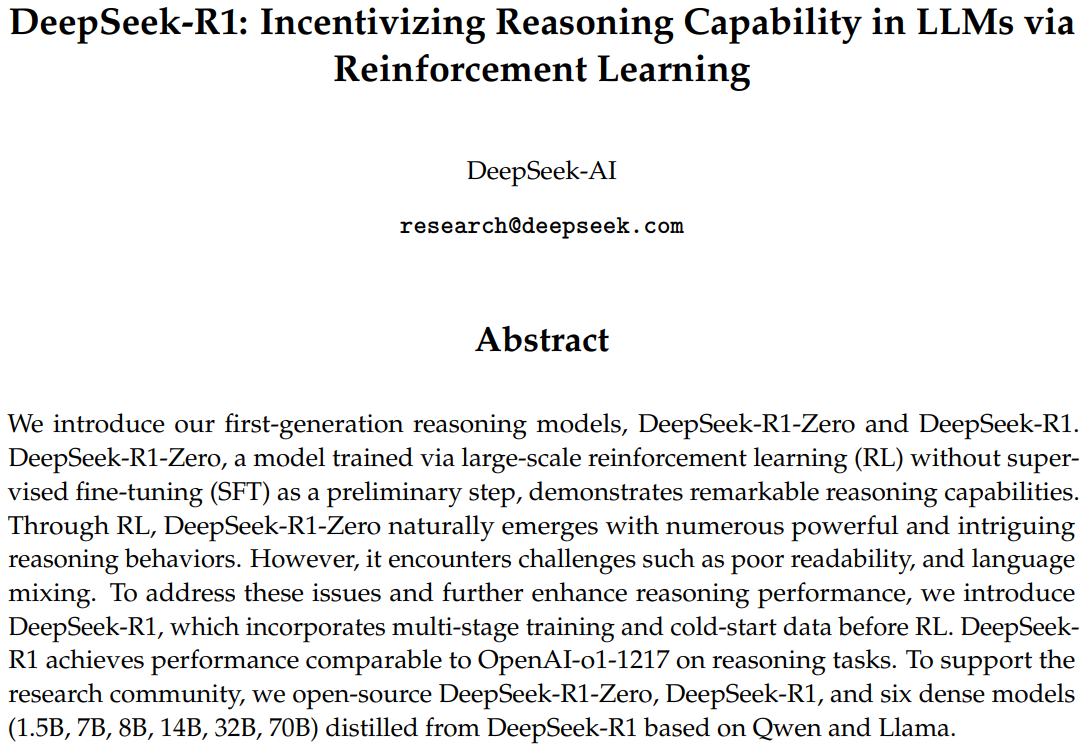
\includegraphics[height=0.9\textheight,width=\textwidth,keepaspectratio]{images/lrm+moe/paper-deepseek-r1.png}
    \end{figure}
    \begin{itemize}
        \item \textbf{What is Reinforcement Learning for Reasoning Skill Refinement?}
        \begin{itemize}
            \item A method to enhance reasoning skills in LLMs through reinforcement learning.
            \item Focuses on refining the model's ability to perform reasoning tasks.
        \end{itemize}
        \item \textbf{How does it work?}
        \begin{itemize}
            \item Uses a reward signal to guide the model towards better reasoning performance.
            \item Involves training the model on a variety of reasoning tasks with feedback.
        \end{itemize}
    \end{itemize}
    
    \framebreak
    \begin{itemize}
        \item \textbf{Why is it important?}
        \begin{itemize}
            \item Enhances the model's reasoning capabilities, making it more effective for complex tasks.
            \item Addresses the limitations of traditional training methods by focusing on skill refinement.
        \end{itemize}
        \item \textbf{Challenges}
        \begin{itemize}
            \item Requires a well-defined reward signal to effectively guide the learning process.
            \item Balancing exploration and exploitation during training can be difficult.
        \end{itemize}
    \end{itemize}
    \framebreak
    \textbf{Examples of Models Using Reinforcement Learning for Reasoning Skill Refinement} 
        \begin{itemize}
            \item \textbf{Deepseek-R1}
            \begin{itemize}
                \setlength{\itemsep}{1em}
                \item Deepseek-R1 utilizes reinforcement learning from human feedback (RLHF) to enhance its reasoning skills.
                \item The model is trained on a variety of reasoning tasks, receiving feedback to iteratively refine its logical and step-by-step problem-solving abilities.
                \item \textit{Example:} Deepseek-R1 can tackle complex reasoning questions by learning from feedback on its intermediate reasoning steps as well as final answers.
            \end{itemize}
        \framebreak
            \begin{figure}[h]
                \centering
                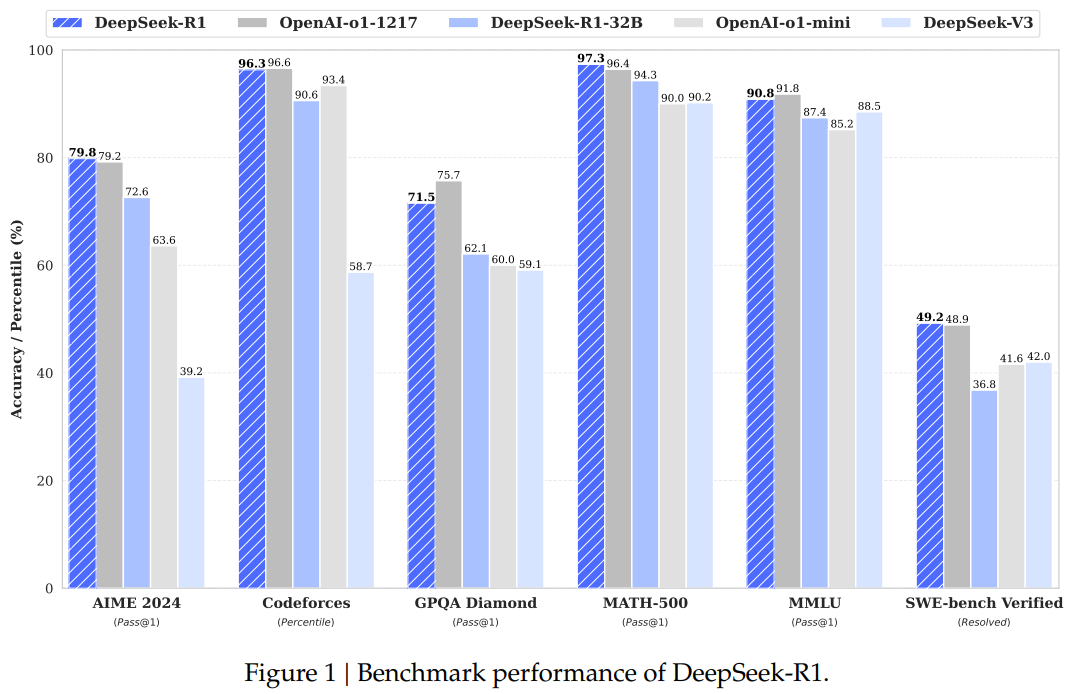
\includegraphics[width=\textwidth,height=0.84\textheight,keepaspectratio]{images/lrm+moe/deepseek-r1-benckmark-performance.png}
                \caption*{Source: \href{https://arxiv.org/pdf/2501.12948}{DeepSeek-AI (2025)}}
            \end{figure}
        \framebreak
            \item \textbf{Llama with RLHF}
            \begin{itemize}
                \setlength{\itemsep}{1em}
                \item Llama models are fine-tuned using RLHF to refine their reasoning and decision-making skills.
                \item RLHF helps Llama models generate more accurate and contextually relevant responses in complex reasoning scenarios.
                \item \textit{Example:} Llama can be trained to provide detailed justifications for its answers in logical deduction tasks.
            \end{itemize}
        \framebreak
            \item \textbf{GPT-4 with RLHF}
            \begin{itemize}
                \setlength{\itemsep}{1em}
                \item GPT-4 uses RLHF extensively to align its outputs with human preferences, especially for tasks requiring nuanced reasoning.
                \item The model is exposed to a wide range of reasoning challenges and receives feedback to iteratively improve its performance.
                \item \textit{Example:} GPT-4 can engage in Socratic dialogue, refining its reasoning through interactive feedback.
            \end{itemize}
        \framebreak
            \item \textbf{Other Models}
            \begin{itemize}
                \setlength{\itemsep}{1em}
                \item Many recent LLMs (e.g., PaLM, Claude) incorporate RLHF or similar reinforcement learning techniques to enhance reasoning.
                \item These models benefit from iterative feedback and reward signals tailored to reasoning skill development.
            \end{itemize}
        \end{itemize}
    \framebreak
        \begin{figure}[h]
            \centering
            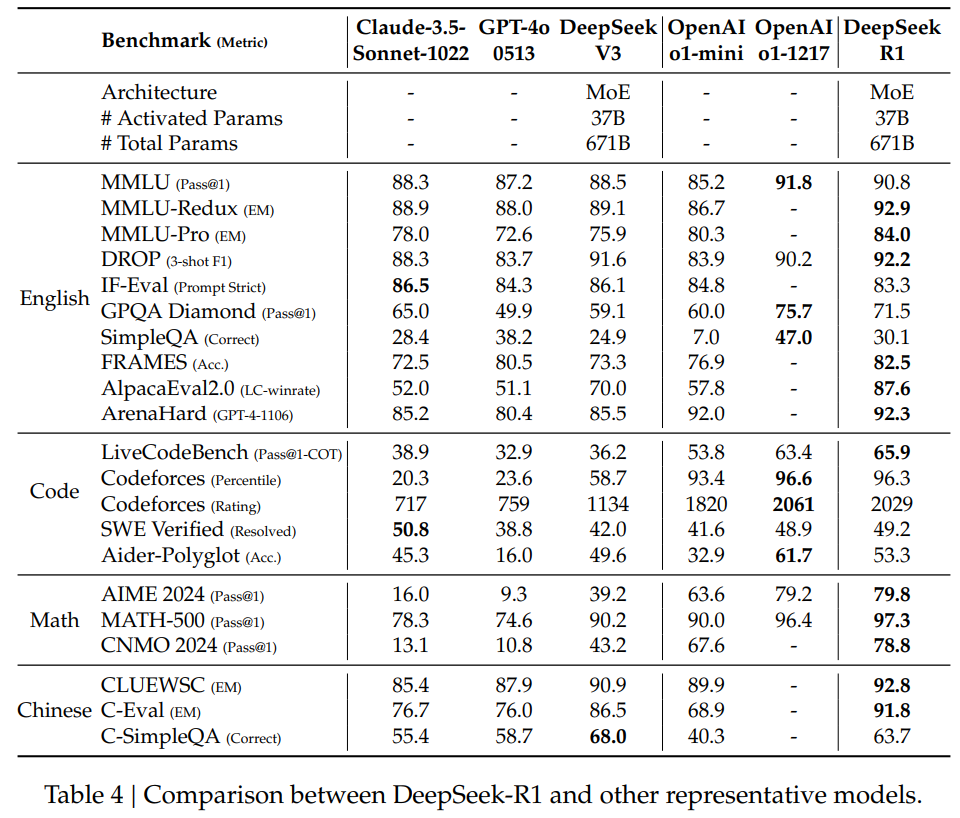
\includegraphics[width=\textwidth,height=0.84\textheight,keepaspectratio]{images/lrm+moe/deepseek-r1-evaluation.png}
            \caption*{Source: \href{https://arxiv.org/pdf/2501.12948}{DeepSeek-AI (2025)}}
        \end{figure}
    \framebreak
        \begin{figure}[h]
            \centering
            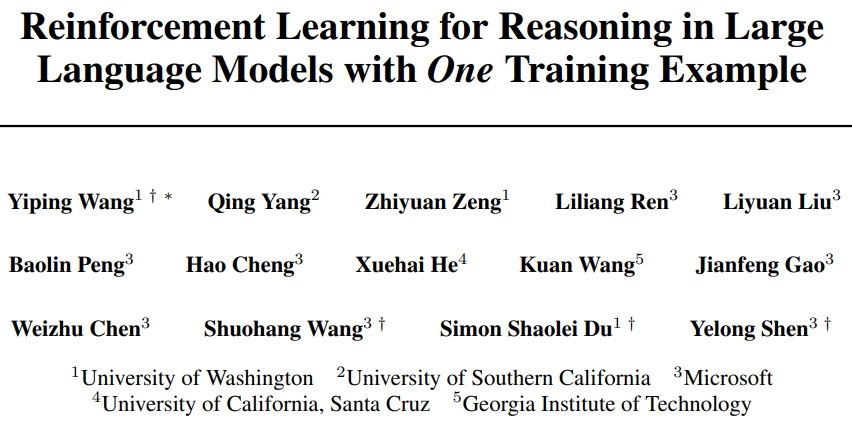
\includegraphics[width=\textwidth,height=0.84\textheight,keepaspectratio]{images/lrm+moe/paper-rl-for-reasoning-llm.png}
            \caption*{Source: \href{https://arxiv.org/pdf/2504.20571}{Wang et al. (2025)}}
        \end{figure}
    \framebreak
        \begin{figure}[h]
            \centering
            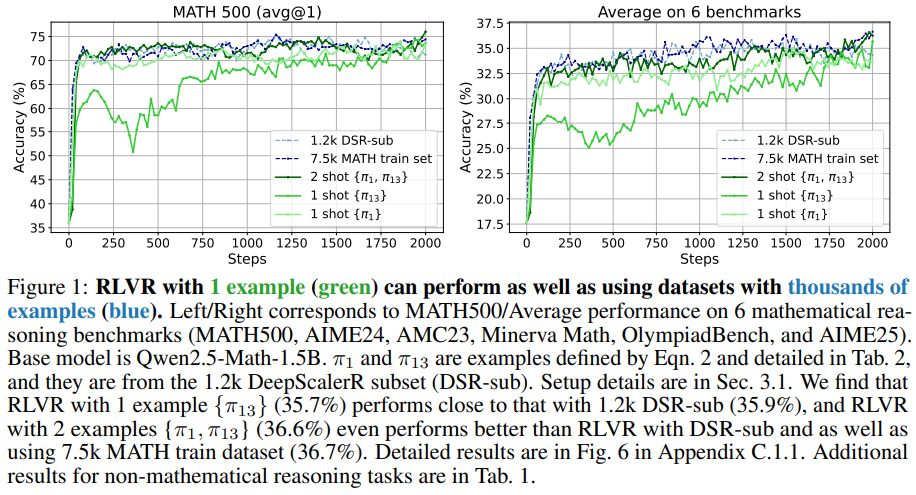
\includegraphics[width=\textwidth,height=0.84\textheight,keepaspectratio]{images/lrm+moe/rlvr-dataset-result.png}
            \caption*{Source: \href{https://arxiv.org/pdf/2504.20571}{Wang et al. (2025)}}
        \end{figure}
    \framebreak
        \begin{figure}[h]
            \centering
            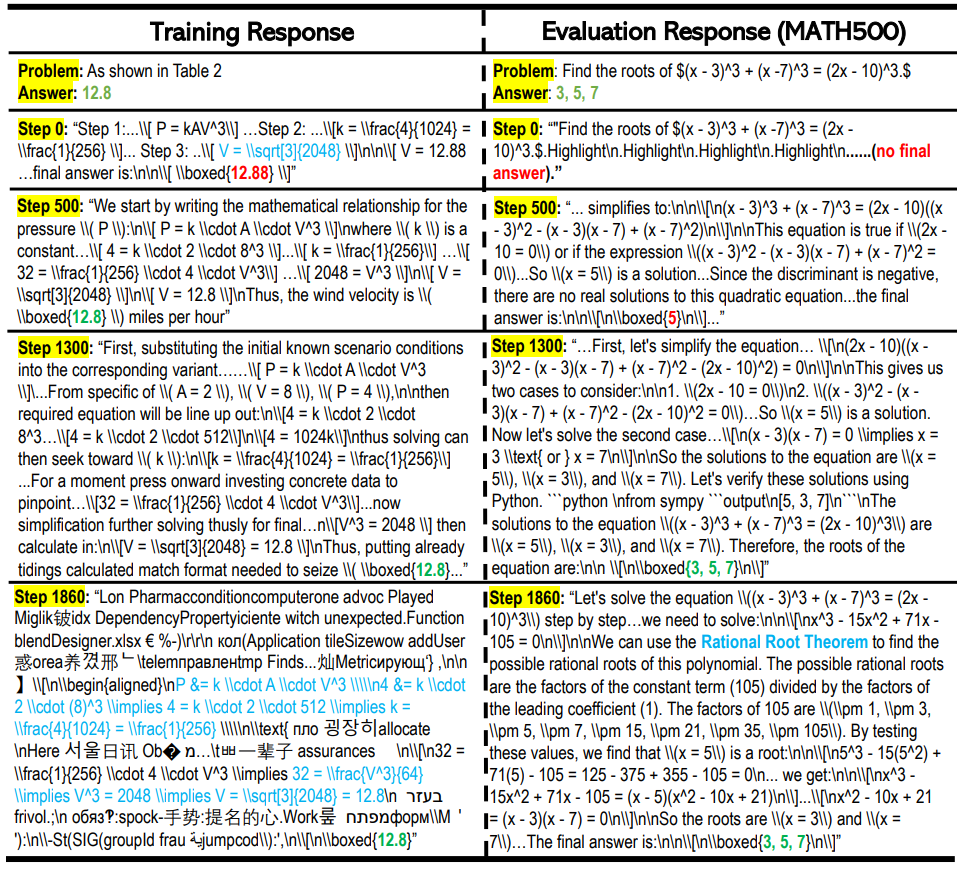
\includegraphics[width=\textwidth,height=0.78\textheight,keepaspectratio]{images/lrm+moe/rlvr-result.png}
            \caption*{Model’s response to training example π1 and a selected MATH500 problem. Green/Red are used for marking Correct/Wrong answers. Source: \href{https://arxiv.org/pdf/2504.20571}{Wang et al. (2025)}}
        \end{figure}
    \framebreak
        \begin{figure}[h]
            \centering
            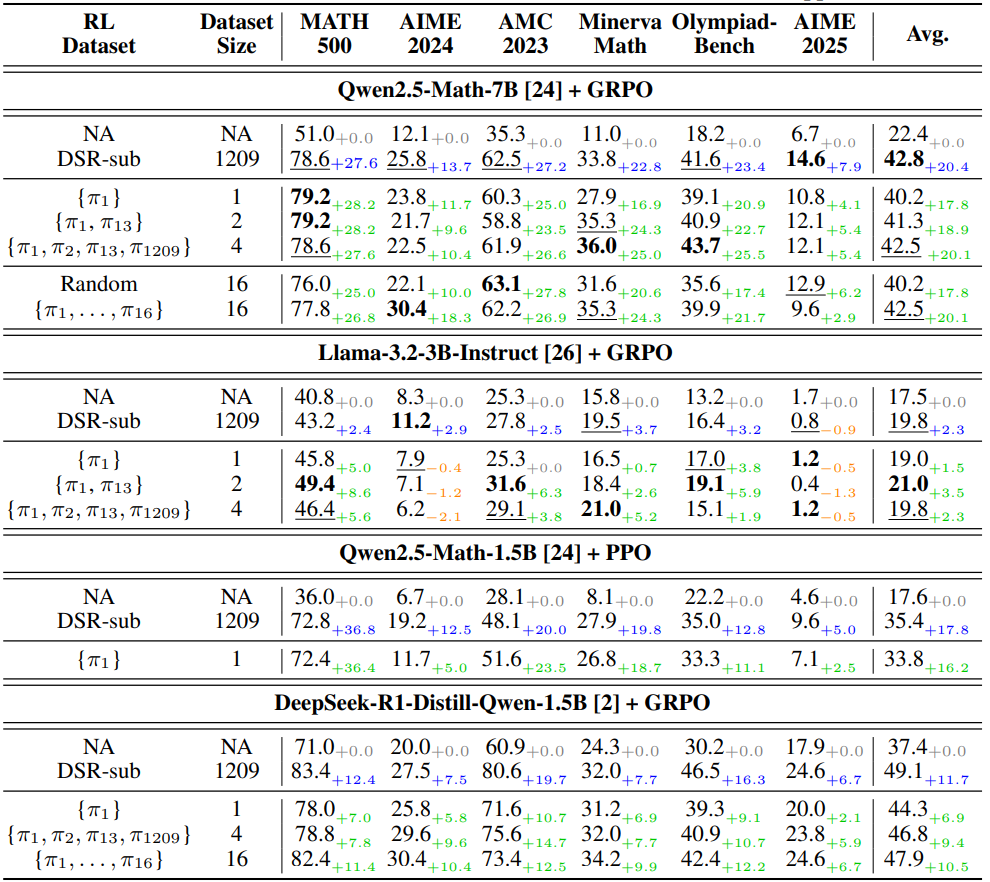
\includegraphics[width=\textwidth,height=0.84\textheight,keepaspectratio]{images/lrm+moe/rlvr-viability.png}
            \caption*{1(few)-shot RLVR is viable for different models and RL algorithm. Source: \href{https://arxiv.org/pdf/2504.20571}{Wang et al. (2025)}}
        \end{figure}
    \framebreak
    \begin{itemize}
        \item \textbf{Applications}
        \begin{itemize}
            \item Can be applied to various reasoning tasks, such as logical reasoning, mathematical problem solving, and decision-making.
            \item Useful in scenarios where reasoning skills are critical for task success.
        \end{itemize}
        \item \textbf{Advanced Techniques}
        \begin{itemize}
            \item Combining a reward model with a verifier model to ensure both performance and correctness.
            \item Rewarding attributes such as truthfulness, logical soundness, or helpfulness during training.
        \end{itemize}
        \item \textbf{Future Directions}
        \begin{itemize}
            \item Further research is needed to improve the efficiency and effectiveness of reinforcement learning for reasoning skill refinement.
            \item Exploring different reward structures and training paradigms to enhance model performance.
        \end{itemize}
    \end{itemize}
\end{frame}